\section{Auswertung}
\label{sec:auswertung}

\subsection{Eichung der Messanlage}
Für die Eichung der Messanlagen wurden Messungen der Frequenzspektren von verschiedenen Ketten aus Zylinderresonatoren aufgenommen. Die Messung wurde mit dem Computer aufgenommen. Die Ergenisse sind in 
Abbildung \ref{fig:zyl1-6-12} dargestellt. 
\begin{figure}[H]
    \centering
    \begin{tabular}{c}
      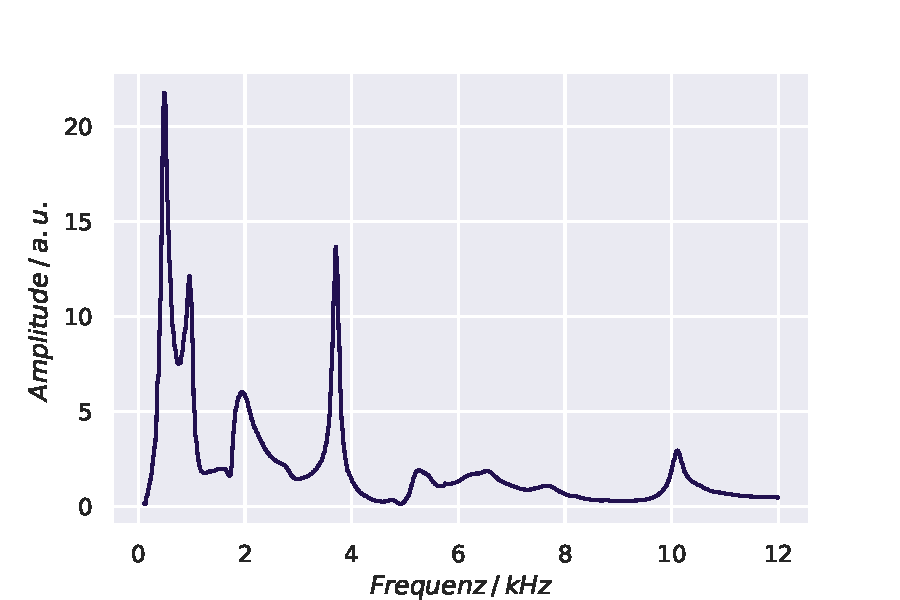
\includegraphics[width=0.7\textwidth]{Daten/Zyinder/Zylinder_1.pdf} \\
    (a) 1 Zylinder \\[6pt]
     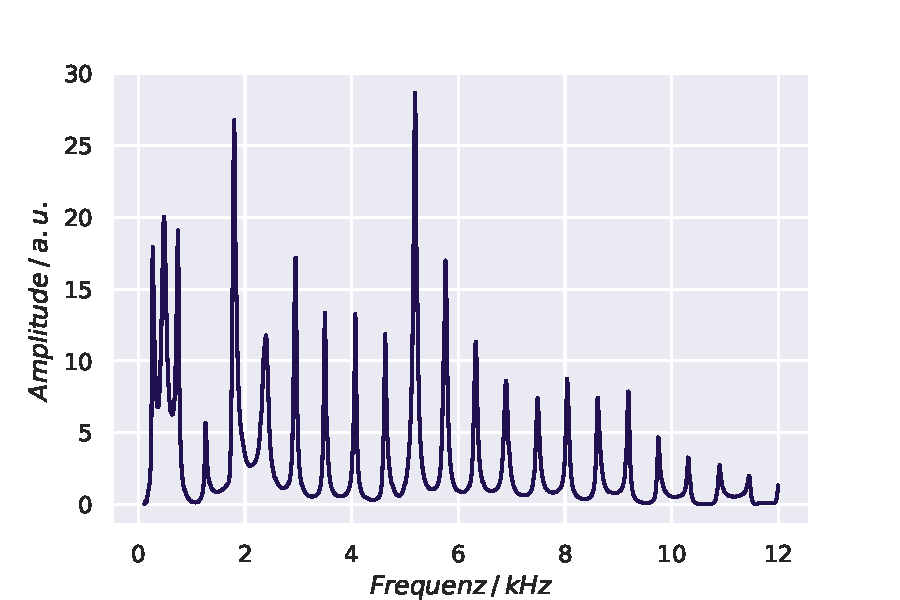
\includegraphics[width=0.7\textwidth]{Daten/Zyinder/Zylinder_6.pdf} \\
    (b) 6 Zylinder \\[6pt]
    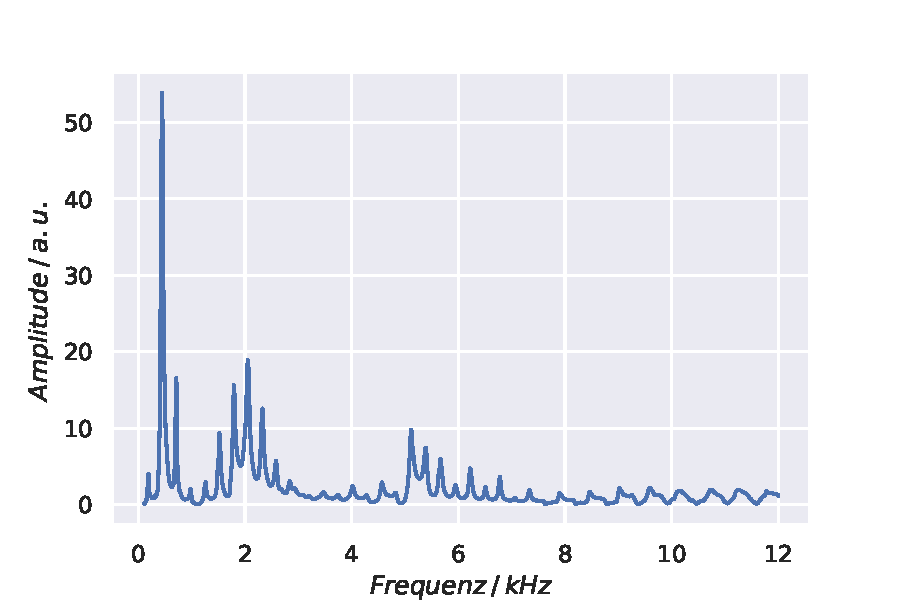
\includegraphics[width=0.7\textwidth]{Daten/Zyinder/Zylinder_12.pdf} \\
    (c) 12 Zylinder \\[6pt]
    \end{tabular}
    \caption{Gemessene Frequenzspektren der Zylinder-Resonatoren mit unterschiedlicher Länge. } 
    \label{fig:zyl1-6-12}
\end{figure}

Die Messungen mit dem Oszilloskop zeigen den selben Verlauf wie die Messungen mit dem Computer. Es ist bei allen Messungen das charakteristische Spektrum eines Festkörpers ersichtlich. Die einzelnen Peaks geben die Resonanzen wieder der Zylinderkette. Wie erwartet, nimmt auch die Amplitude mit steigender Frequenz ab. 
Somit bestätigen die Messungen insgesamt die Erwartungen und die Eichung war damit erfolgreich. 
Es ist zu erwähnen, dass die Messung des einzelnen Zylinders ersichtlich nur unsauber gelungen ist. Hier sind die Resonanzen des Zylinders nicht eindeutig erkennbar. Für die weiteren Messungen sind jedoch scharfe Peaks an den Resonanzfrequenzen zu erkennen. \\
Hieran anschließend, wurde das Spektrum eines Zylinders der Länge $75\,\si{\milli\metre}$ aufgenommen. Das Spektrum ist in der Abbildung \ref{fig:fkp75mm} zu sehen.

\begin{figure}[H]
    \centering
    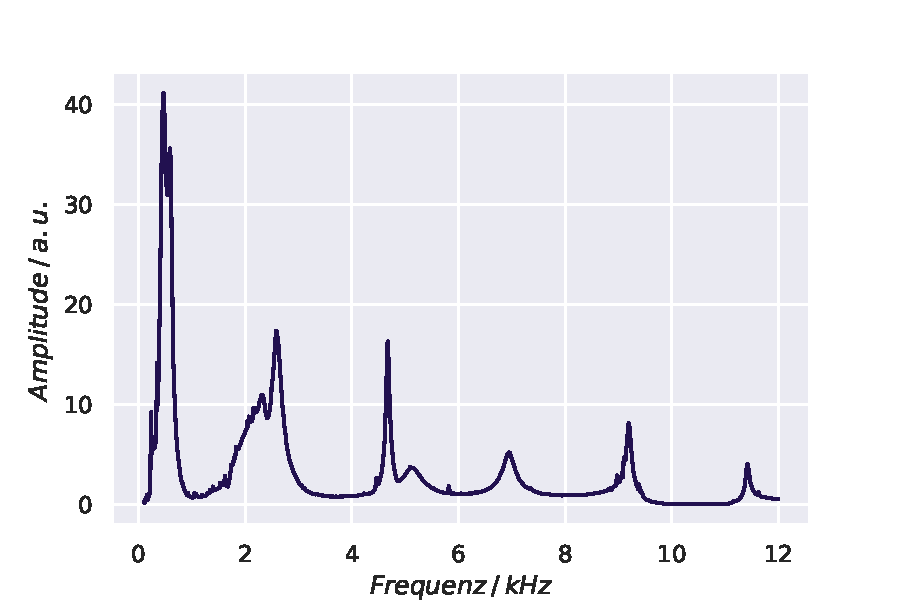
\includegraphics[width=0.8\textwidth]{Daten/Festkörper/FK_75mm.pdf}
    \caption{Das Frequenzspektrum eines $75 \,\si{\milli\metre}$ langen Zylinder-Resonators. }
    \label{fig:fkp75mm}
\end{figure}
An diesem Spektrum sind periodisch auftretende Resonanzen ersichtlich. Die Resonanzen des $75 \,\si{\milli\metre}$ Zylinders müssen an den Frequenzen auftreten, die ca. $\frac{2}{3}$ der Resonanzfrequenzen des $50 \,\si{\milli\metre}$ Zylinders entsprechen. 
Dies folgt aus der größeren Länge des Zylidners. Die stehende Welle des $75 \,\si{\milli\metre}$ Zylinders hat die $1.5$-fache Wellenlänge der stehenden Welle des $50 \,\si{\milli\metre}$ Zylinders. Die Frequenz ist umgekehrt proportional zur Wellenlänge und damit folgt der Faktor $\frac{2}{3}$.

\subsection{Das Wasserstoffatom}
Das Frequenzspektrum des Kugelresonators bei einer Ausrichtung von $\alpha = 180°$ wurde mit dem Computer aufgenommen und in der Abbildung \ref{fig:h180} grafisch dargestellt. 
Die beschrifteten Resonanzen werden in der folgenden Analyse für die Berechnung der Druckamplitude verwendet. 
\begin{figure}[H]
    \centering
    \begin{tabular}{c}
    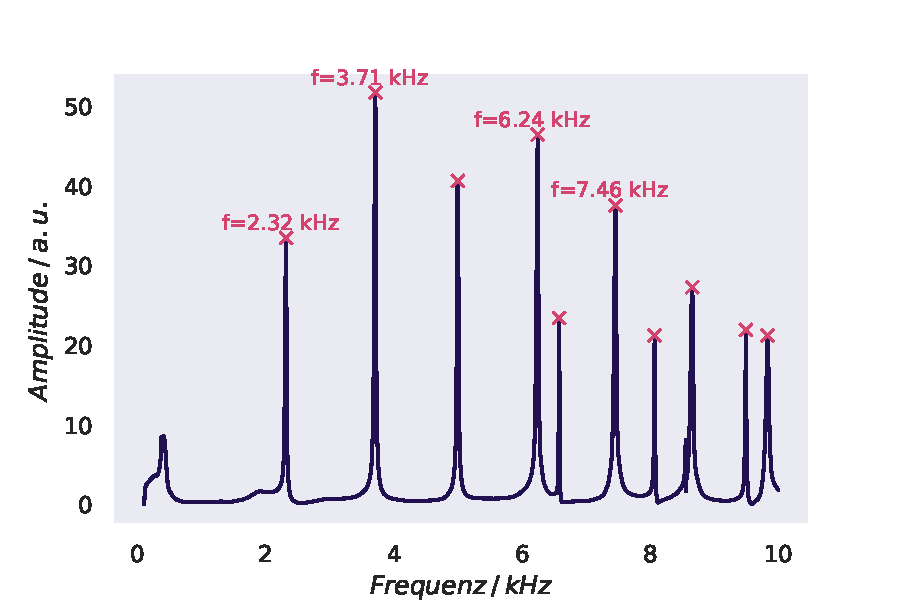
\includegraphics[width=0.9\textwidth]{Daten/Wasserstoff/neu/H_180.pdf} \\
    (a) Messung am Computer \\[6pt]
    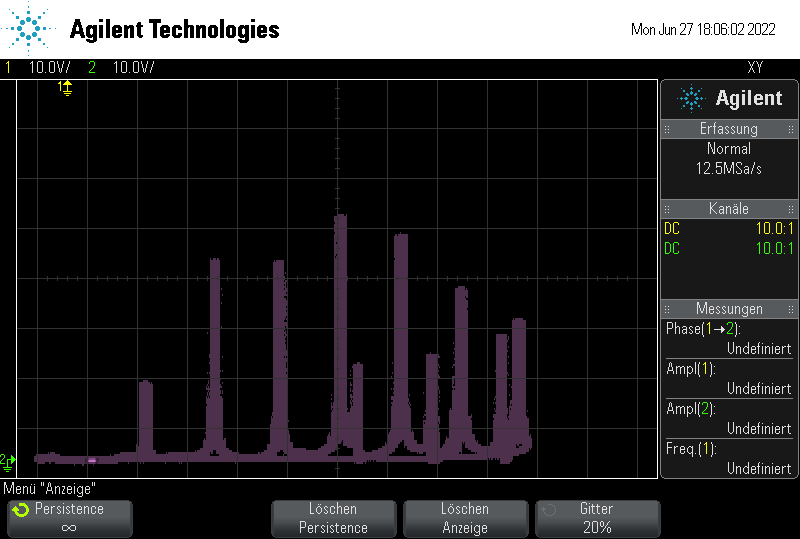
\includegraphics[width=0.9\textwidth]{Daten/Oszilloskop/scope_4.png} \\
    (b) Messung am Oszilloskop \\[6pt]
    \end{tabular}
    \caption{Das Frequenzspektrum eines kugelförmigen Hohlraumresonators bei einer Ausrichtung von $\theta = 180\si{°}$ in dem Bereich $0.1 \,\si{\kilo\hertz}$ bis $10 \,\si{\kilo\hertz}$. }
    \label{fig:h180}
\end{figure}

\subsubsection{Druckamplitude}
Für die Berechnung der Druckamplitude mithilfe der gemessenen Werte wird der Ausrichtungswinkel $\alpha$ folgendermaßen in den Polarwinkel $\varphi$ umgerechnet:
\begin{align*}
  \varphi = \arccos(\frac{1}{2} \cos(\alpha) - \frac{1}{2}).
\end{align*}
Diese Umrechnung folgt aus einer Analyse mit Drehmatrizen \cite{qa-dresden}. Die in Abbildung \ref{fig:h180} beschrifteten Resonanzfrequenzen (also $2.32 \,\si{\hertz}$, $3.71 \,\si{\hertz}$, $6.24 \,\si{\hertz}$ und $7.46 \,\si{\hertz}$) werden nur in Abhängigkeit der Auslenkung in $10°$-Schritten erneut gemessen. Für diese Messung werden bei jeder Auslenkung die Position der Peaks erneut bestimmt und die Höhe abgelesen. 
Die Messung wird in Abhängigkeit des Polarwinkels in Abbildung \ref{fig:hpeaks} aufgetragen. In der selben Abbildung befindet sich der theoretisch erwartete Verlauf bzw. die entsprechenden Legendrepolynome. 
\begin{figure}[H]
  \centering
  \begin{tabular}{cc}
    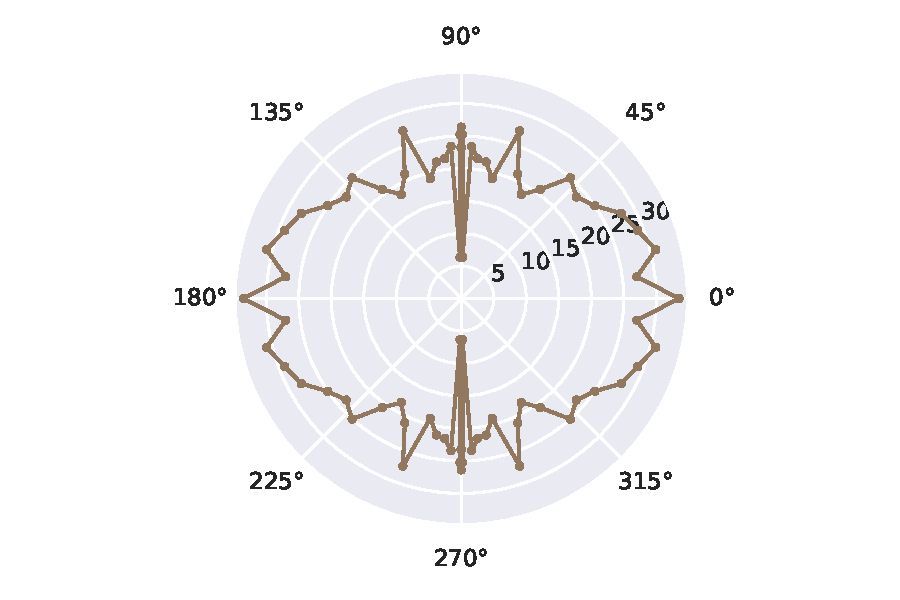
\includegraphics[width=0.5\textwidth]{Daten/Wasserstoff/neu/peak0.pdf} &   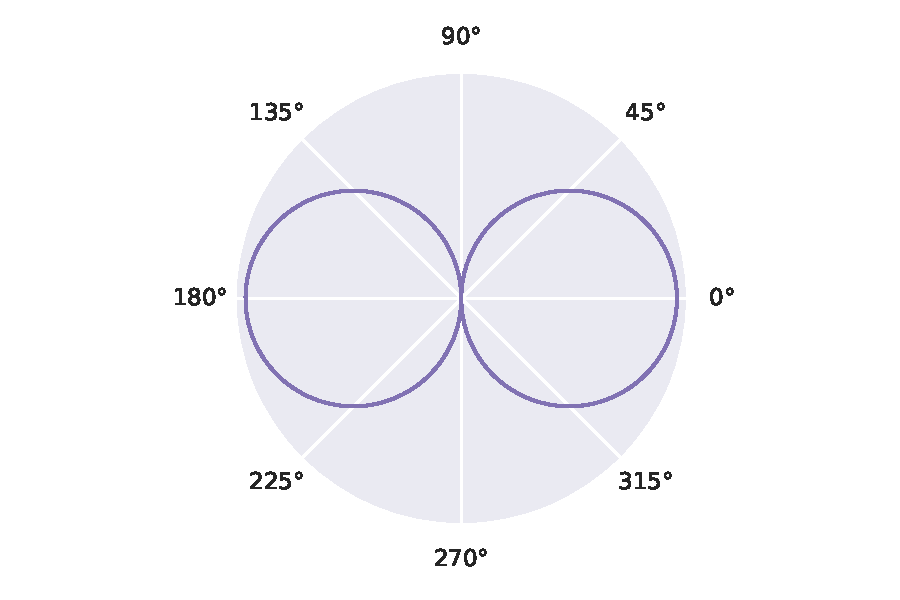
\includegraphics[width=0.5\textwidth]{Daten/Wasserstoff/peakLeg0.pdf} \\
  (a) Resonanz bei $2.32 \,\si{\kilo\hertz} $& (b) $P_1(\cos(\theta))$ \\[6pt]
  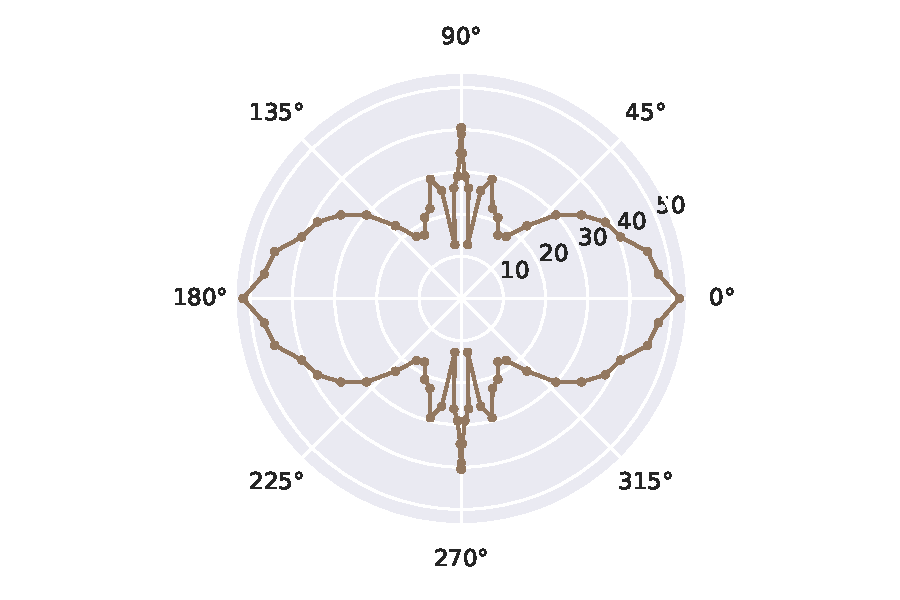
\includegraphics[width=0.5\textwidth]{Daten/Wasserstoff/neu/peak1.pdf} &   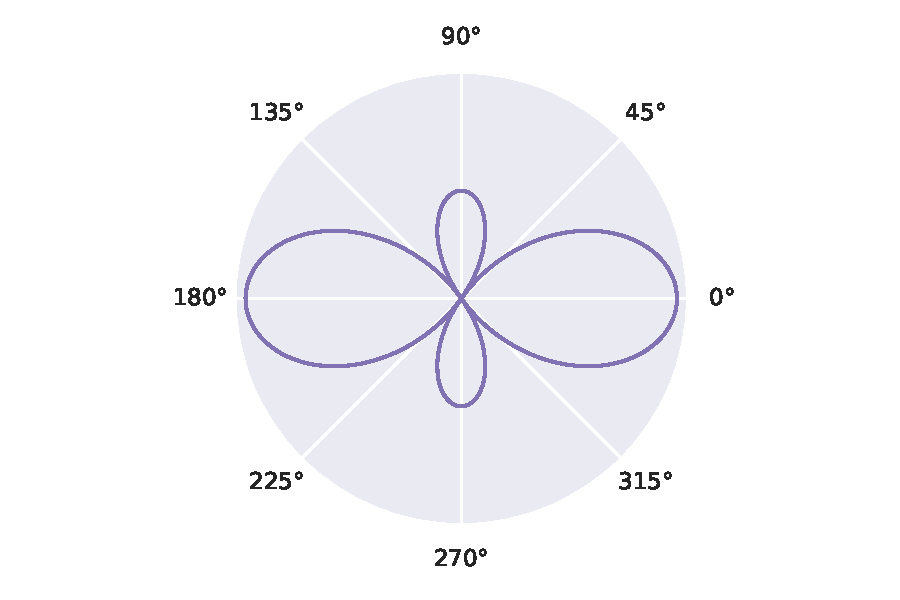
\includegraphics[width=0.5\textwidth]{Daten/Wasserstoff//peakLeg1.pdf} \\
  (c) Resonanz bei $3.71 \,\si{\kilo\hertz}$ & (d) $P_2(\cos(\theta))$ \\[6pt]
  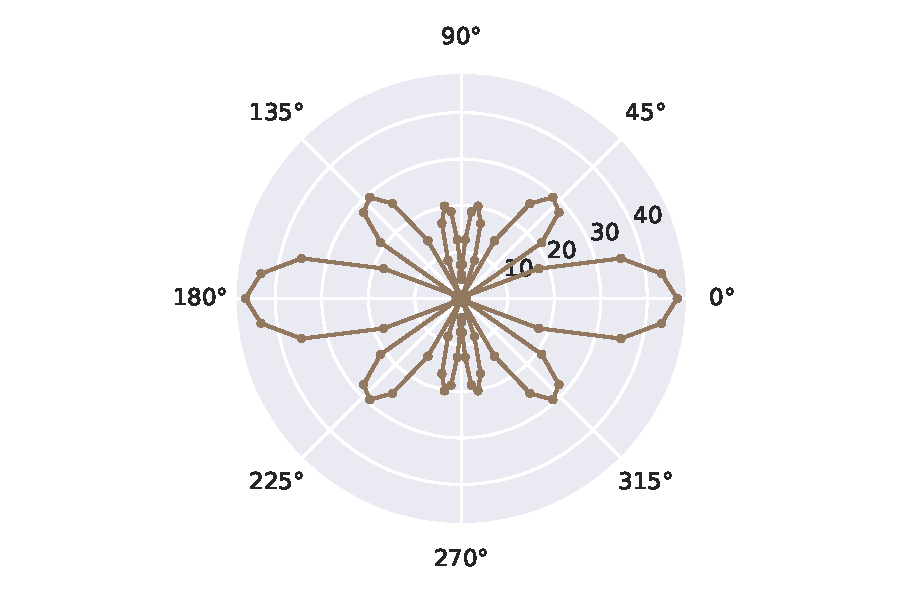
\includegraphics[width=0.5\textwidth]{Daten/Wasserstoff/neu/peak2.pdf} &   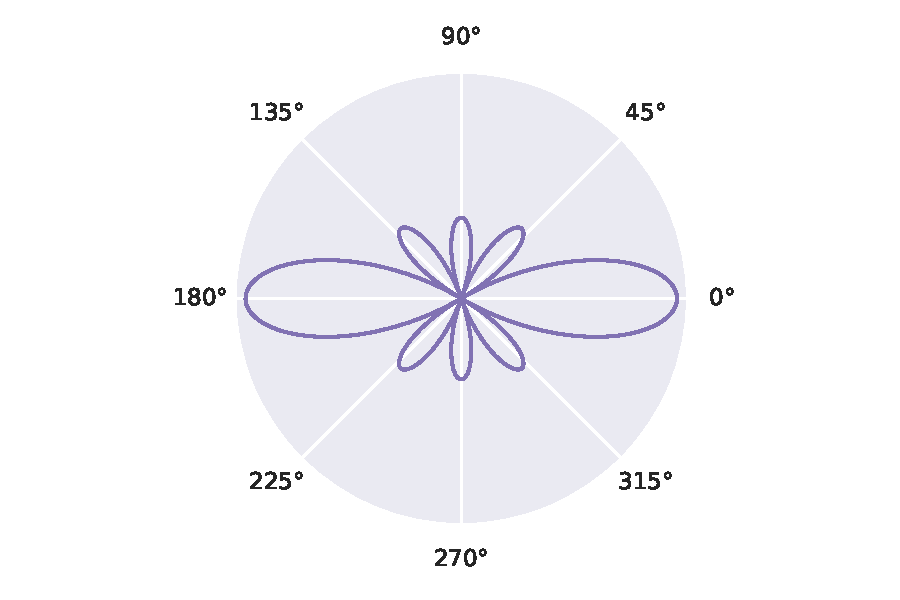
\includegraphics[width=0.5\textwidth]{Daten/Wasserstoff/peakLeg2.pdf} \\
  (c) Resonanz bei $6.24 \,\si{\kilo\hertz}$ & (d) $P_4(\cos(\theta))$ \\[6pt]
  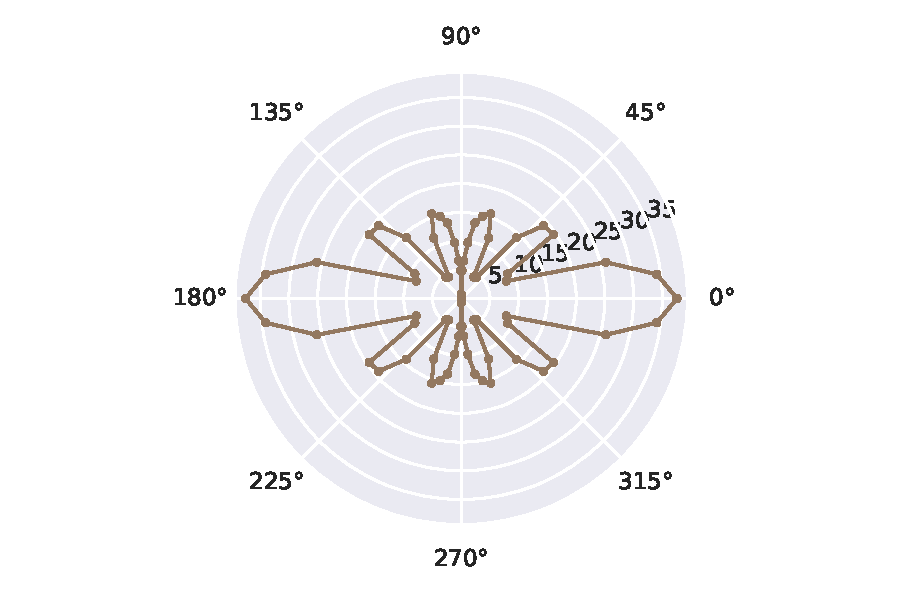
\includegraphics[width=0.5\textwidth]{Daten/Wasserstoff/neu/peak3.pdf} &   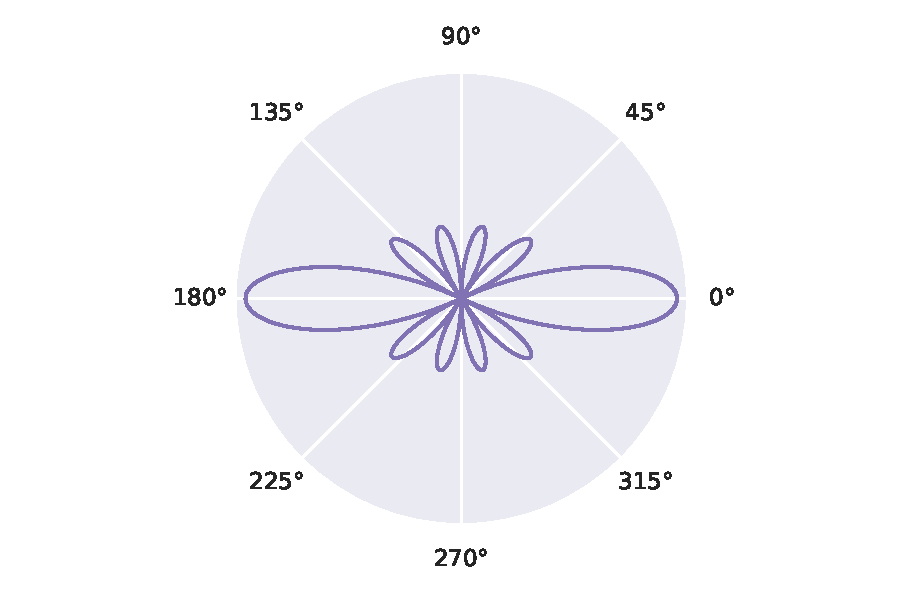
\includegraphics[width=0.5\textwidth]{Daten/Wasserstoff/peakLeg3.pdf} \\
  (c) Resonanz bei $7.46 \,\si{\kilo\hertz}$ & (d) $P_5(\cos(\theta))$ \\[6pt]
  
  \end{tabular}
  \caption{Amplitudenmessung an den Resonanzfrequenzen in Abhängigkeit vom Azimutwinkel $\phi$ neben der passenden Legendrepolynome. } 
  \label{fig:hpeaks}
\end{figure}
\subsubsection{Aufspaltung der Peaks}
In diesem Abschnitt werden die Frequenzspektren um die Resonanz bei $2.3 \,\si{\kilo\hertz}$ bei einer Ausrichtung von $\alpha = 0°$ aufgenommen mit Blenden verschiedener Dicke aufgenommen. Das Ergebnis sind in den Abbildungen \ref{fig:hspalt} dargestellt. 
Die Resonanz spaltet sich in zwei Peaks auf, da die Kugelsymmetrie des Resonators durch die Blenden gebrochen wird. Der Abstand der Peaks ist ungefähr proportional zur Dicke der Blenden.
\begin{figure}[H]
  \centering
  \begin{tabular}{cc}
    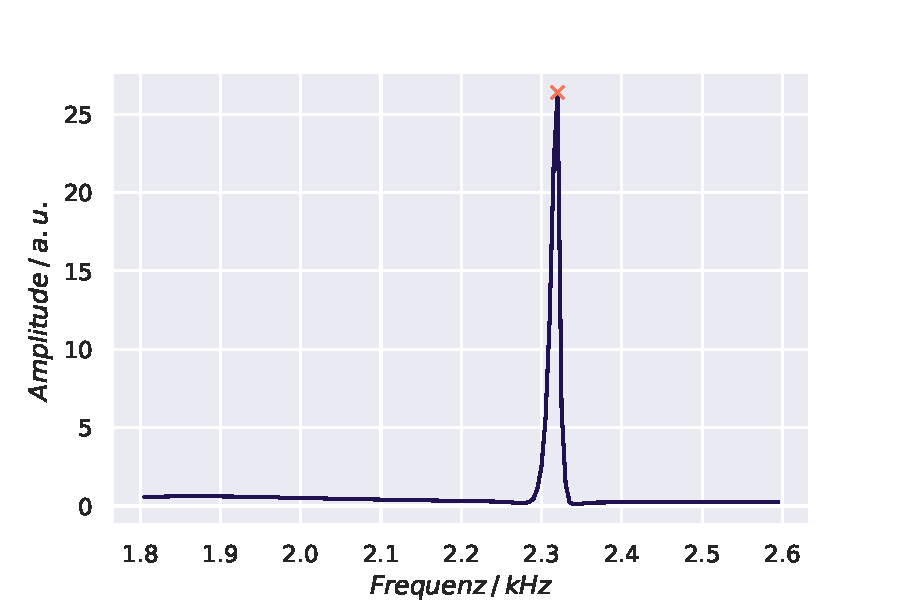
\includegraphics[width=0.5\textwidth]{Daten/Wasserstoff/neu/spalt0.pdf} &   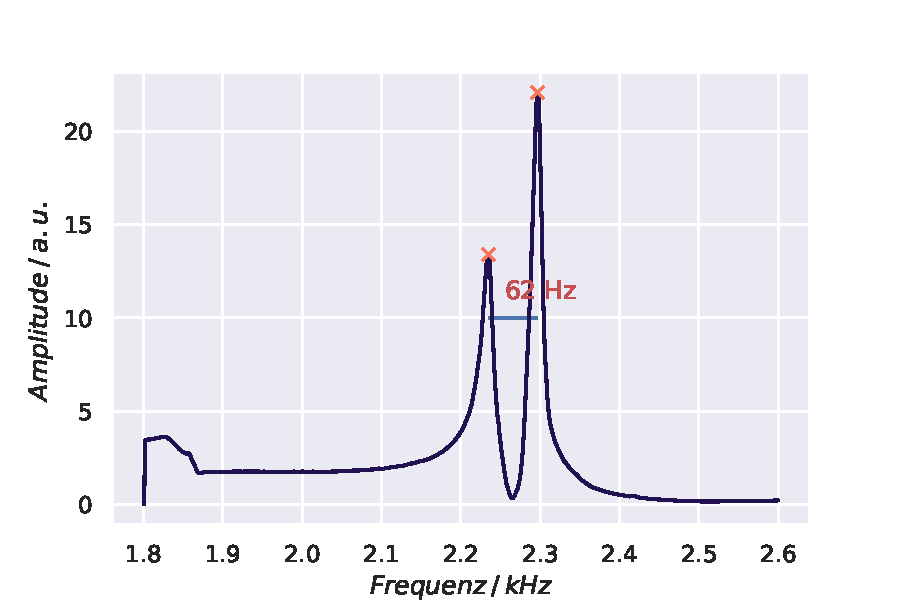
\includegraphics[width=0.5\textwidth]{Daten/Wasserstoff/neu/spalt1.pdf} \\
  (a) Ohne Ring & (b) $3 \,\si{\milli\metre}$ Ring \\[6pt]
  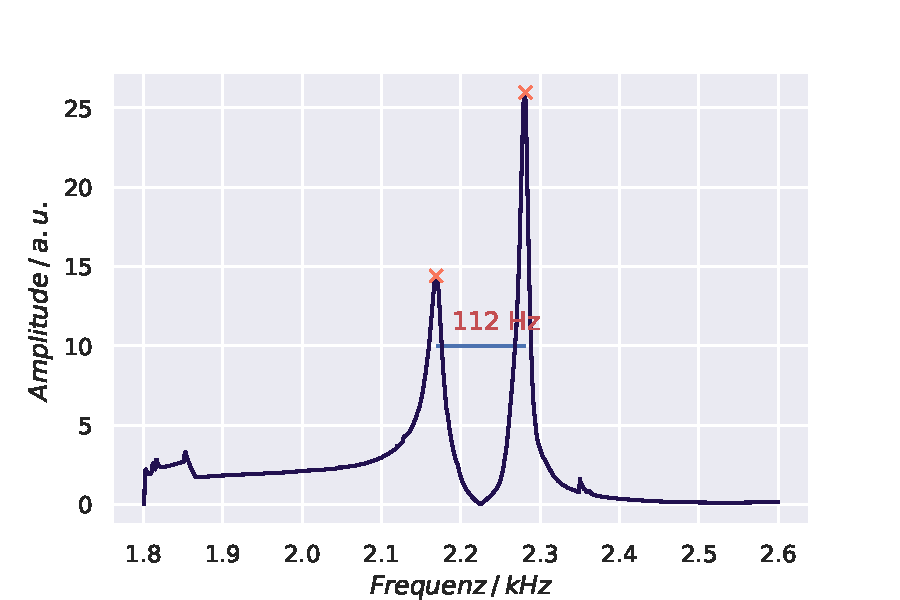
\includegraphics[width=0.5\textwidth]{Daten/Wasserstoff/neu/spalt2.pdf} &   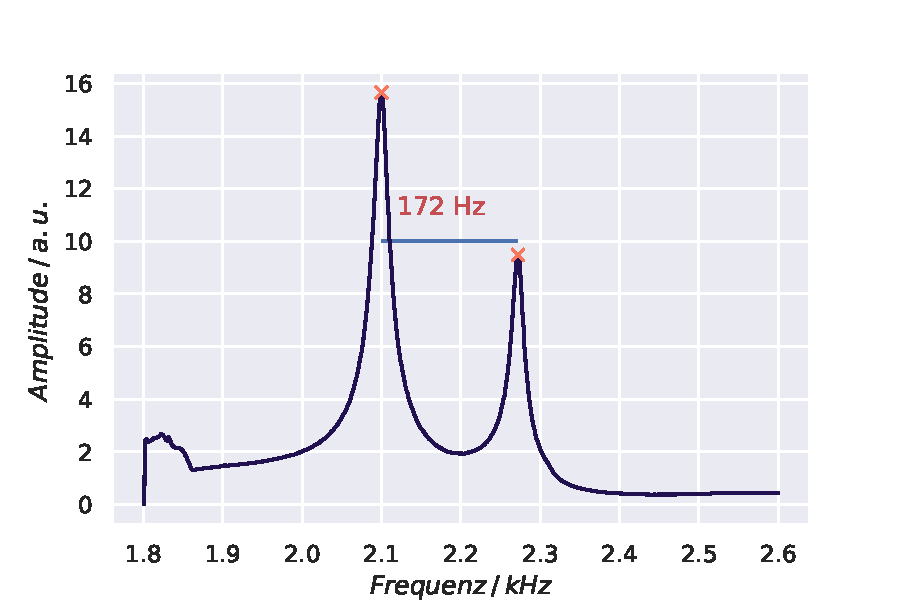
\includegraphics[width=0.5\textwidth]{Daten/Wasserstoff/neu/spalt3.pdf} \\
  (c)  $6 \,\si{\milli\metre}$ Ring & (d)  $9 \,\si{\milli\metre}$ Ring \\[6pt]
  \multicolumn{2}{c}{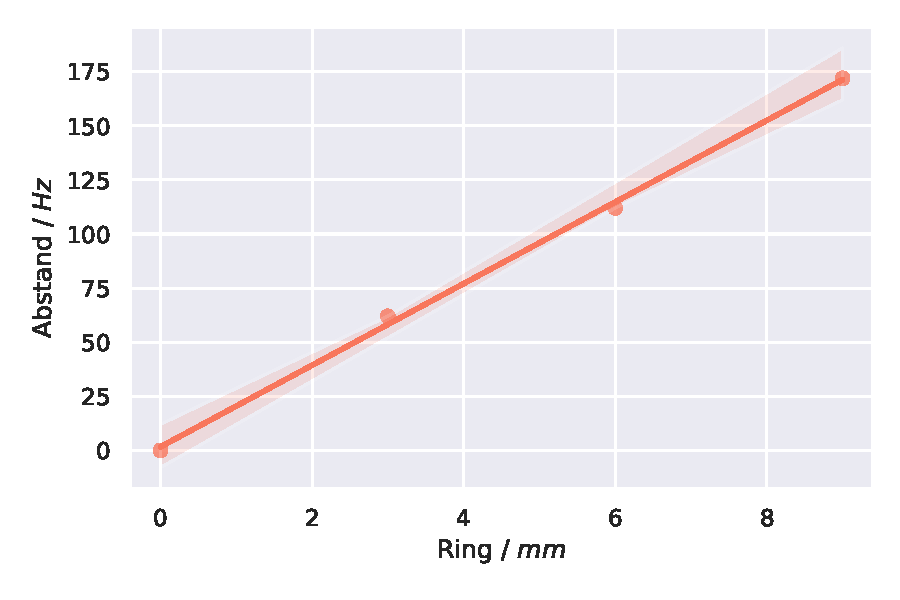
\includegraphics[width=0.65\textwidth]{Daten/Wasserstoff/neu/spaltGesamt.pdf}}\\[6pt]
  \multicolumn{2}{c}{(e) Abstand in Abhängigkeit von der Blendendicke.}
  \end{tabular}
  \caption{Aufspaltung des Peaks bei $2.3 \,\si{\kilo\hertz}$ nachdem verschiedene Ringe die Kugelsymmetrie brechen. Der Schatten gibt die Unsicherheit des Fits wieder. } 
  \label{fig:hspalt}
\end{figure}
\subsubsection{Druckamplitude mit der $9 \,\si{\milli\metre}$ Blende}
Die Druckamplitude wurde um die beiden Peaks bei $2.08 \,\si{\kilo\hertz}$ und $2.25 \,\si{\kilo\hertz}$ in der Abbildung \ref{fig:9mm} aufgezeichnet. Die zugehörigen Legendrepolynome sind ebenfalls in der Abbildung zu sehen. Aus Abbildung \ref{fig:hpeaks} ist bekannt, dass ohne Zwischenring hier der Zustand $l=1$ liegt. Mit Zwischenring gibt es also eine Aufspaltung dieses Zustands. 
Die $2.08 \,\si{\kilo\hertz}$ Resonanz weist daher auf den Zustand $l=1$ und $m=0$ und die $2.25 \,\si{\kilo\hertz}$ Resonanz weist auf den Zustand $l=1$ und $m=\pm 0$ hin. Der Vergleich mit den Legendrepolynomen ist ebenfalls in der Abbildung \ref{fig:9mm} zu sehen. 
\begin{figure}[H]
  \centering
  \begin{tabular}{cc}
    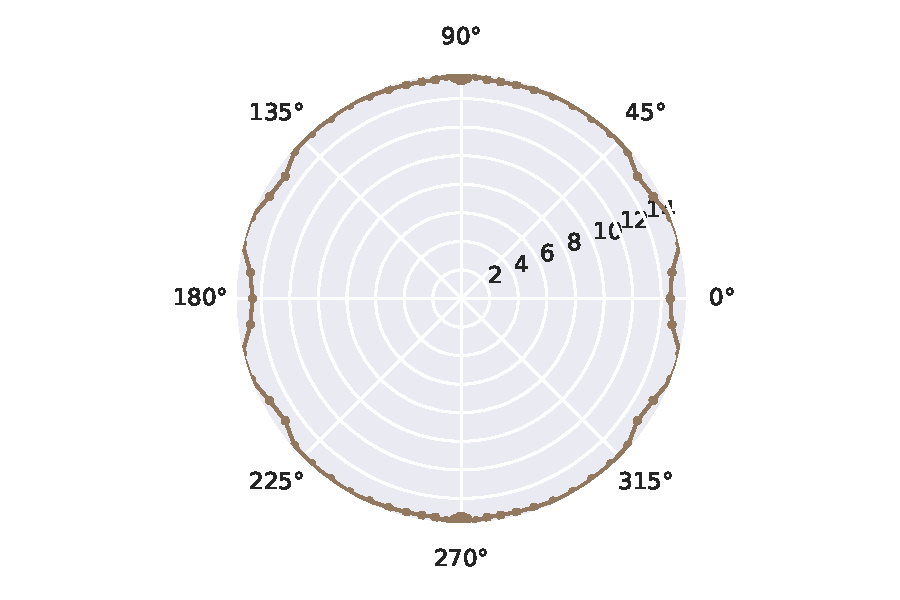
\includegraphics[width=0.5\textwidth]{Daten/Wasserstoff/neu/peak9mm1.pdf} &   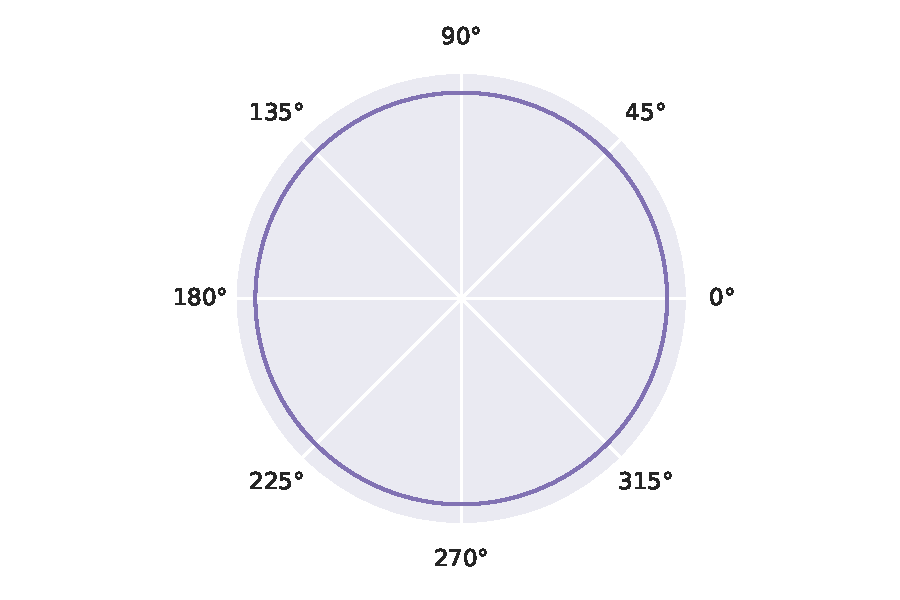
\includegraphics[width=0.5\textwidth]{Daten/Wasserstoffmolekuelion/peakLeg.pdf} \\
  (a) $2.10 \,\si{\kilo\hertz}$ Resonanz & (b) $P_0(\cos(\theta))$ \\[6pt]
  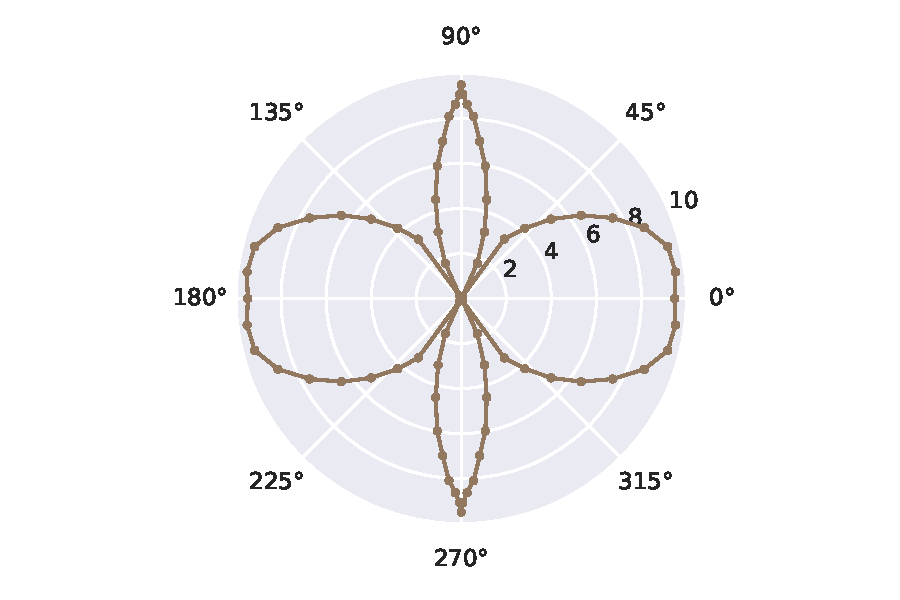
\includegraphics[width=0.5\textwidth]{Daten/Wasserstoff/neu/peak9mm.pdf} &   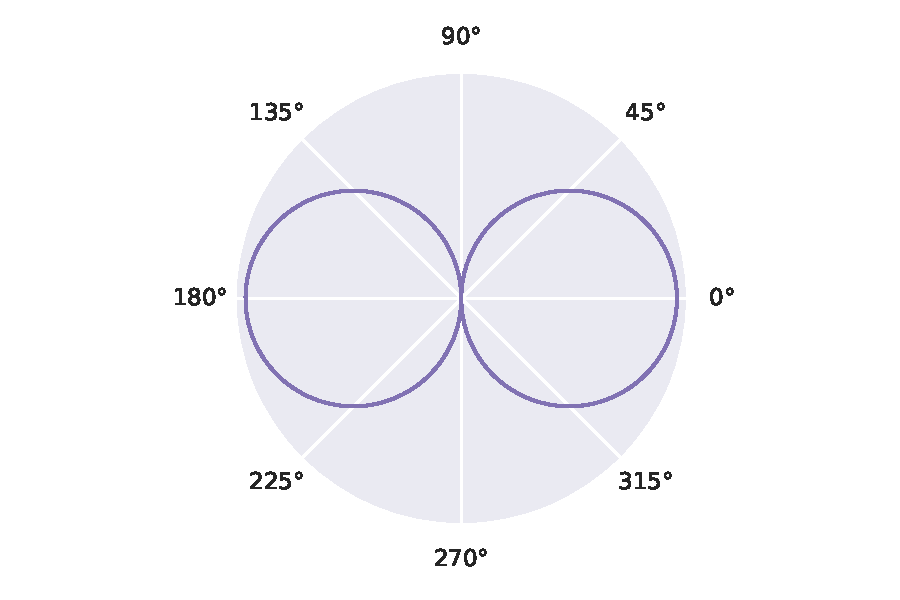
\includegraphics[width=0.5\textwidth]{Daten/Wasserstoff/peakLeg0.pdf} \\
  (c) $2.27 \,\si{\kilo\hertz}$ Resonanz & (d) $P_1(\cos(\theta))$ \\[6pt]
  \end{tabular}
  \caption{Gemessene Druckamplitude der $2.27 \,\si{\kilo\hertz}$ und $2.10 \,\si{\kilo\hertz}$ Resonanz mit der $9 \,\si{\milli\metre}$ Blende mit den zugehörigen Legendrepolynomen.} 
  \label{fig:9mm}
\end{figure}
\subsection{Das Wasserstoffmolekül}
\subsubsection{Änderung des Frequenzspektrums in Abhängigkeit des Blendendurchmessers}
\label{sec:h2peaks}
Ein Wasserstoffmolekülion ist anhand zwei gekoppelter Kugelresonatoren modelliert. Die folgenden Messungen wurden mit Blenden verschiedener Durchmesser zwischen den Kugelresonatoren 
aufgenommen. Das Frequenzspektrum dieses gekoppelten Resonators wurde für die Blenden mit $10\,mm$, $15\,mm$, $20\,mm$ und $25\,mm$ Durchmesser gemessen und in der Abbildung \ref{fig:h2} visualisiert. \\\\

\begin{figure}[H]
  \centering
  \begin{tabular}{cc}
    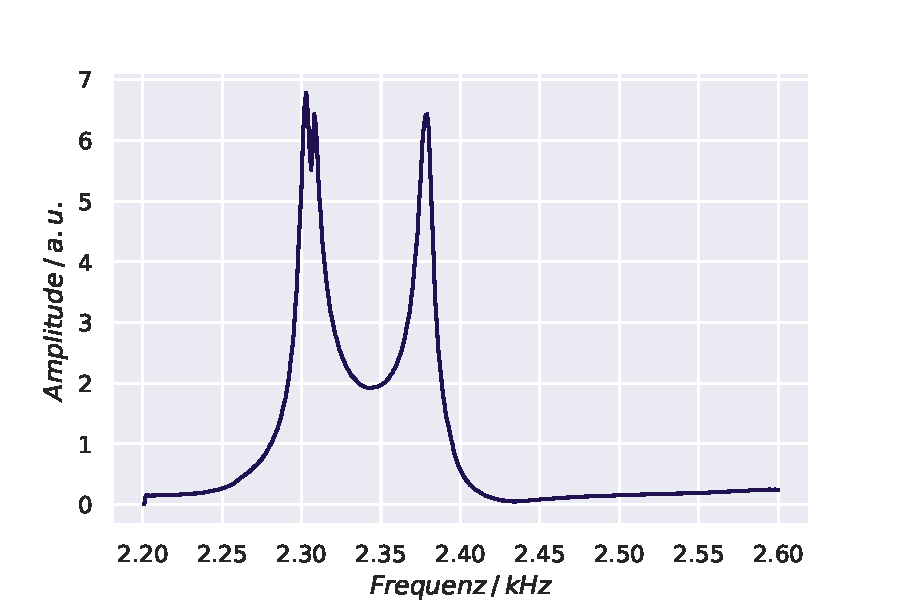
\includegraphics[width=0.5\textwidth]{Daten/Wasserstoffmolekuelion/neu/H2_10mm_180.pdf} &   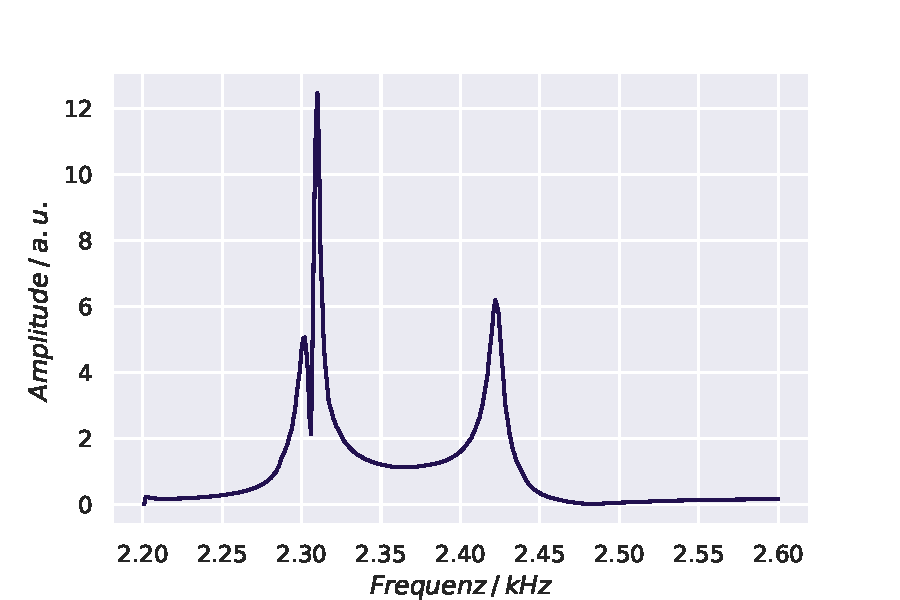
\includegraphics[width=0.5\textwidth]{Daten/Wasserstoffmolekuelion/neu/H2_15mm_180.pdf} \\
  (a) $10 \, \si{\milli\metre}$  & (b) $15 \, \si{\milli\metre}$ \\[6pt]
  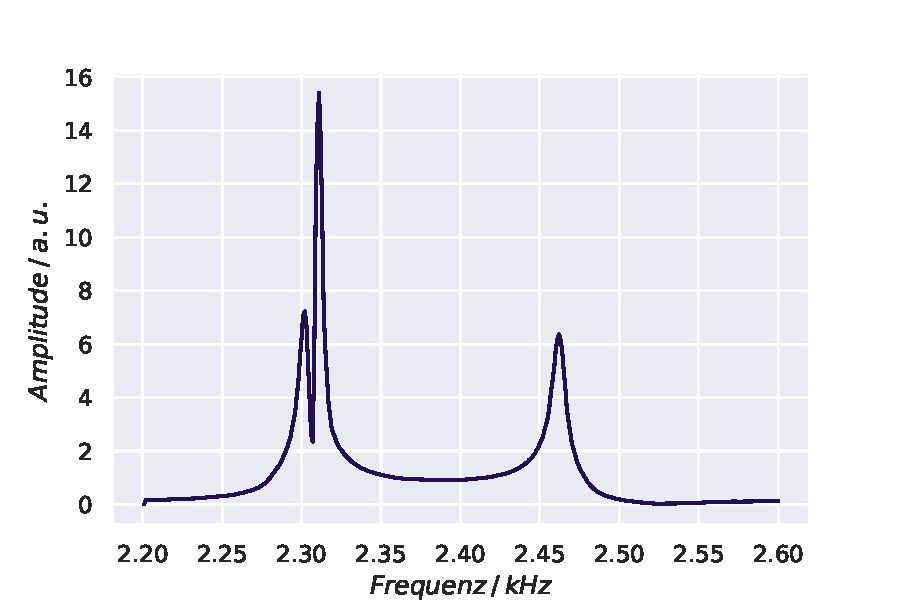
\includegraphics[width=0.5\textwidth]{Daten/Wasserstoffmolekuelion/neu/H2_20mm_180.pdf} &   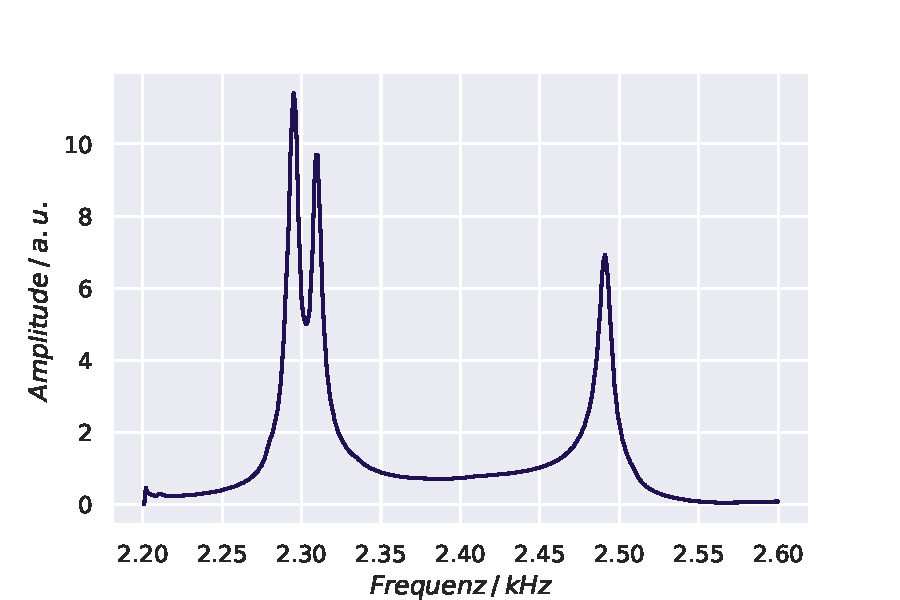
\includegraphics[width=0.5\textwidth]{Daten/Wasserstoffmolekuelion/neu/H2_25mm_180.pdf} \\
  (c)  $20 \, \si{\milli\metre}$ & (d)  $25 \, \si{\milli\metre}$ \\[6pt]
  \multicolumn{2}{c}{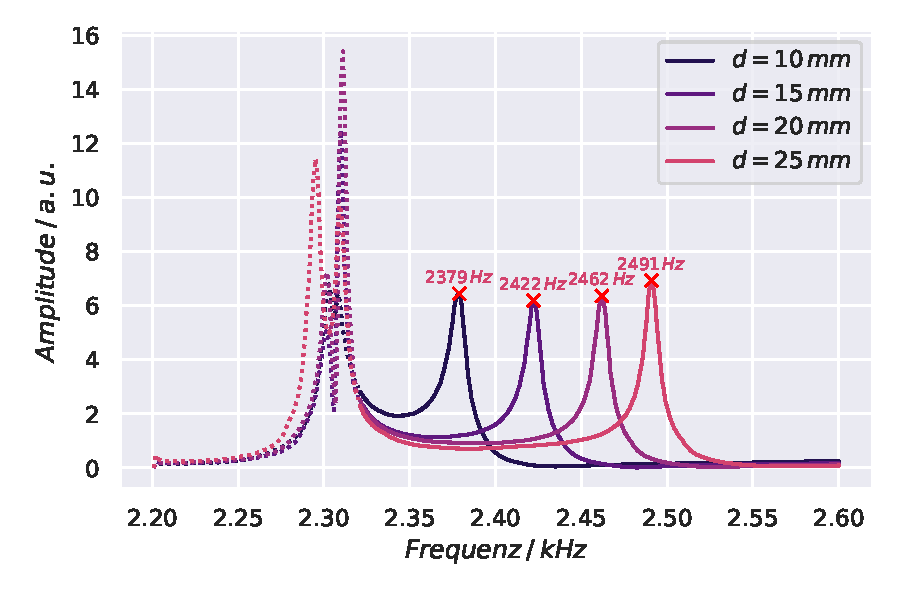
\includegraphics[width=0.65\textwidth]{Daten/Wasserstoffmolekuelion/neu/blendAbhaeng.pdf}}\\[6pt]
  \multicolumn{2}{c}{(e) Vergleich}
  \end{tabular}
  \caption{Frequenzspektren des gekoppelten Resonators in Abhängigkeit der verschiedenen Blendendurchmesser.} 
  \label{fig:h2}
\end{figure}
\begin{figure}[H]
  \centering
  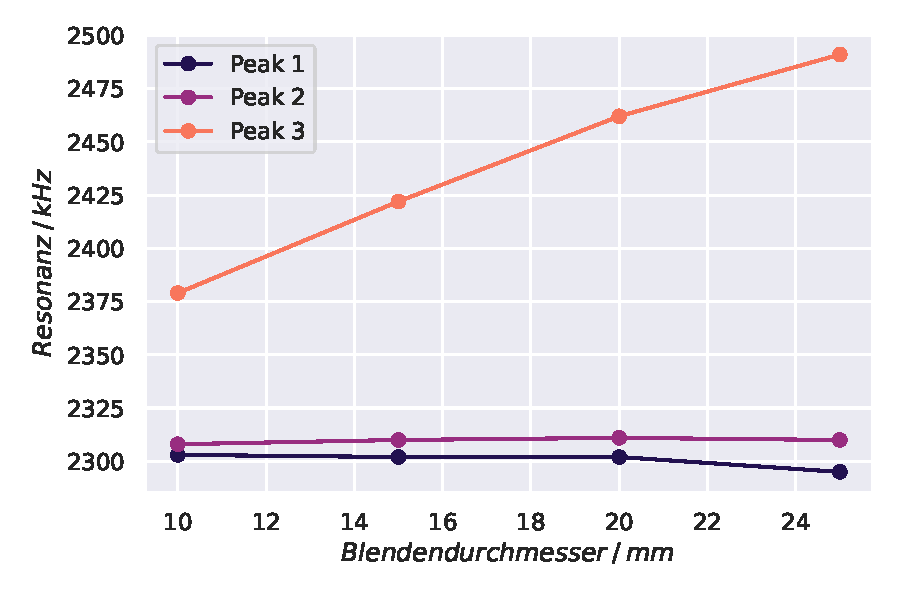
\includegraphics[width=0.8\textwidth]{Daten/Wasserstoffmolekuelion/neu/resonanzBlend.pdf}
  \caption{Resonanzfrequenzen des gekoppelten Resonators in Abhängigkeit der verschiedenen Blendendurchmesser}
  \label{fig:h2Res}
\end{figure}
\subsubsection{Winkelverteilung mit der $25 \, mm$ Blende}
Die Winkelverteilung der drei Peaks aus Abschnitt \ref{sec:h2peaks} wurden in $10°$ Schritten aufgenommen und in der Abbildung \ref{fig:h2_2} wiedergegeben. \\
Peak $1$ und $3$ sind die aufgespaltenen Peaks aus dem Zustand $l=1$, $m=0$ und entsprechen daher den Peaks $2\sigma_g$ und $2\sigma_u$. Die Aufspaltung folgt aus der Austauschwechselwirkung (s. Gleichungen \ref{eqn:wellenfunktion1}-\ref{eqn:wellenfunktion4}). In der Sprache der Bindungstypen entspricht die Bindung dieser Zustände im Wasserstoffmolekülion einer s-Bindung (die Bindungsrichtung entspricht der Symmetrieachse der Schallkörper in den einzelnen Sphären).
Peak $2$ muss demnach aus dem Zustand $l=1$, $m=\pm 1$ hervorgehen. Dies entspricht einer p-Bindung (die Ausrichtung der Symmetrieachse der Schallkörper in den einzelnen Sphären steht senkrecht zur Bindungsrichtung). Auch hier gibt es einen bindenden und antibindenden Zustand aus der Austauschwechselwirkung, aber da die Bindungsstärke der $p$-Bindung deutlich kleiner als die Bindungsstärke der s-Bindung ist, können die beiden Peaks $1\pi_g$ und $1\pi_u$ nicht unterschieden werden (die Frequenzen liegen zu nahe beieinander). 

\begin{figure}[H]
  \centering
  \begin{tabular}{cc}
  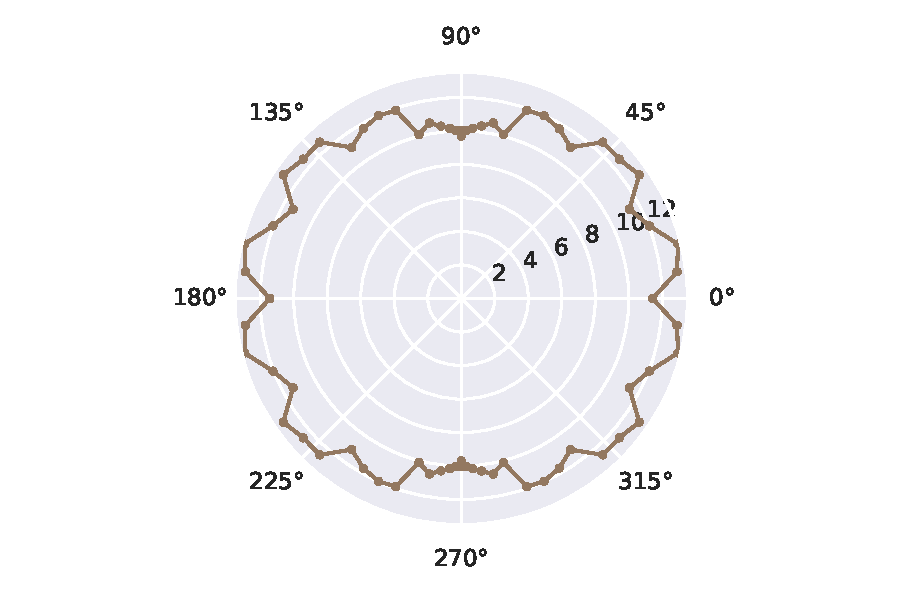
\includegraphics[width=0.5\textwidth]{Daten/Wasserstoffmolekuelion/neu/peak0.pdf} &   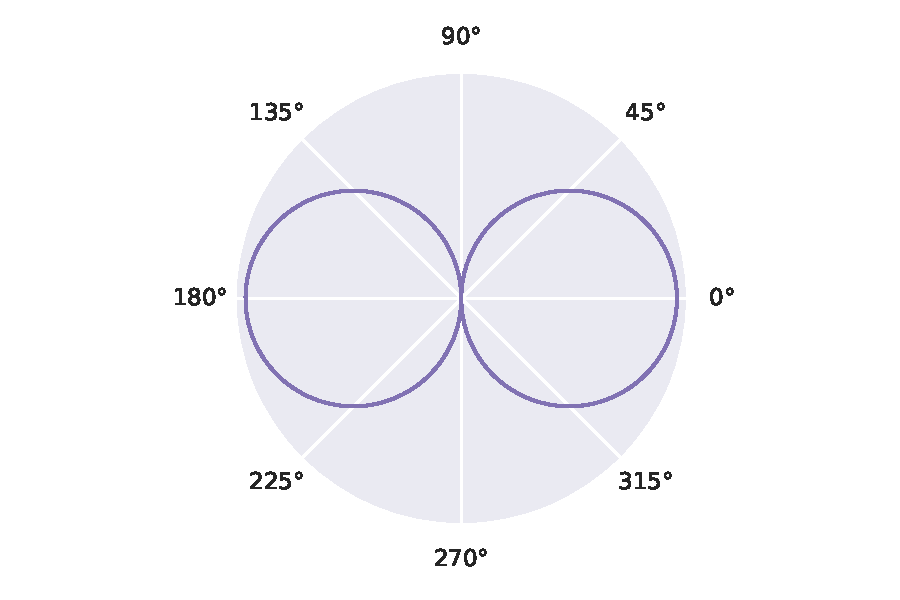
\includegraphics[width=0.5\textwidth]{Daten/Wasserstoff/peakLeg0.pdf}\\[6pt]
  (a)  Peak 1 & (b)  $P_1(\cos(\theta))$ \\[6pt]
  \multicolumn{2}{c}{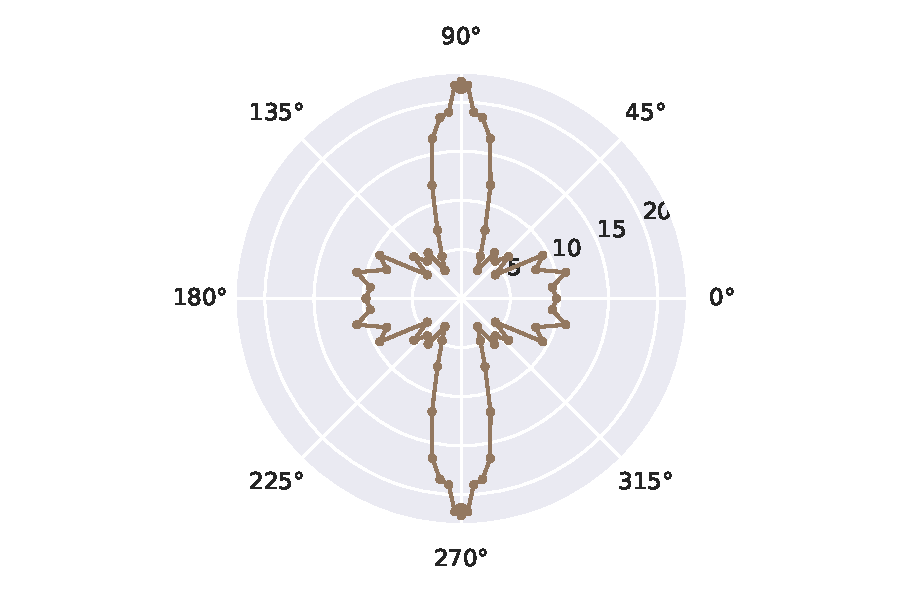
\includegraphics[width=0.5\textwidth]{Daten/Wasserstoffmolekuelion/neu/peak1.pdf}}\\[6pt]
  \multicolumn{2}{c}{(b) Peak 2}\\[6pt]
  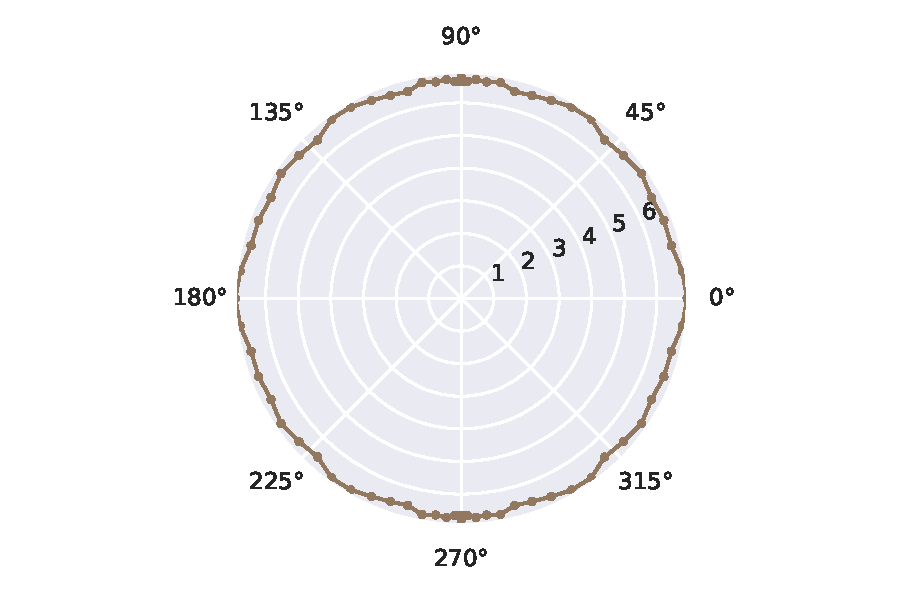
\includegraphics[width=0.5\textwidth]{Daten/Wasserstoffmolekuelion/neu/peak2.pdf} &   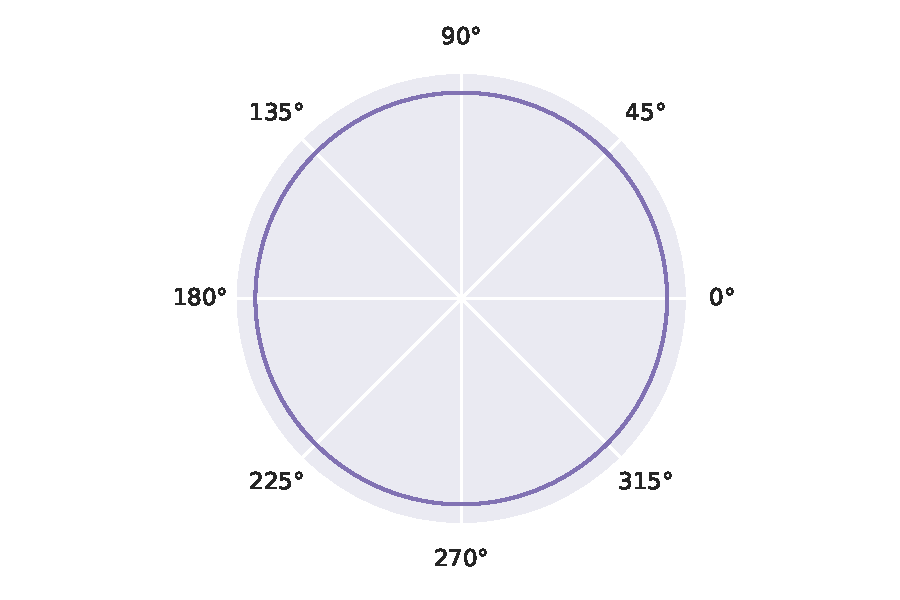
\includegraphics[width=0.5\textwidth]{Daten/Wasserstoffmolekuelion/peakLeg.pdf}\\[6pt]
  (c)  Peak 3 & (d)  $P_0(\cos(\theta))$ \\[6pt]
  \end{tabular}
  \caption{Winkelverteilung des gekoppelten Resonators bei einem Blendendurchmesser von $25\, mm$ mit passenden Legendrepolynomen.} 
  \label{fig:h2_2}
\end{figure}
\subsection{Zylinderketten als Modell für eindimensionale Festkörper}
\subsubsection{Der Übergung von einem Molekül zum Festkörper}
In diesem Abschnitt wurden die Frequenzspektren von Zylinderketten mit einer wachsenden Anzahl an Zylindern gemessen. Die Ergebnisse für Ketten mit $2$,$4$,$6$ und $10$ Zylindern und einem Blendendurchmesser von $16\, mm$ sind in der 
Abbildung \ref{fig:fk1} angegeben.\\
In der Festkörperphysik beschreiben Bänder die dicht beieinander liegende Resonanzfrequenzen der Elektronen in einem Festkörper. Diese entsprechen den Schwingungen welche sich nur wenig von den Eigenschwingungen der anderen Elektronen unterscheiden. 
In dem betrachteten Modell werden diese Schwinungen durch Schallwellen dargestellt. In der Abbildung \ref{fig:fk1} sind deutlich Bänder zu erkennen, welche auch unabhängig von der Anzahl der Zylinder sind. 
Die Bänder selbst werden durch verschiedene stehende Schallwellen im Zylinder erzeugt. Die stehende Welle kann beschrieben werden durch 
\begin{align*}
  \Psi(x) = A\cdot \sin(k_x x),  & \:\:k_x = \frac{2 \pi n_x}{L}
\end{align*}
wobei $A$ die Amplitude angibt und $n_x \in \mathbb{N}$ ist. Das $L$ gibt die Länge der Zylinder an. \\
Die Abbildung \ref{fig:fk1} zeigt, dass die Amplitude der Resonanzfrequenzen mit steigender Frequenz abnimmt. Dies liegt an der Transferfunktion zwischen Lautsprecher und Mikrofon liegen, da der Lautsprecher und das Mikrofon die höhere Frequenzen nicht in gleicher Intensität wiedergeben bzw. aufzeichnen können. 
Dies kann damit erklärt werden, dass höhere Frequenzen höhere Energien benötigen. Damit sinkt die Amplitude aufgrund der Energieerhaltung. 

\begin{figure}[H]
  \centering
  \begin{tabular}{cc}
    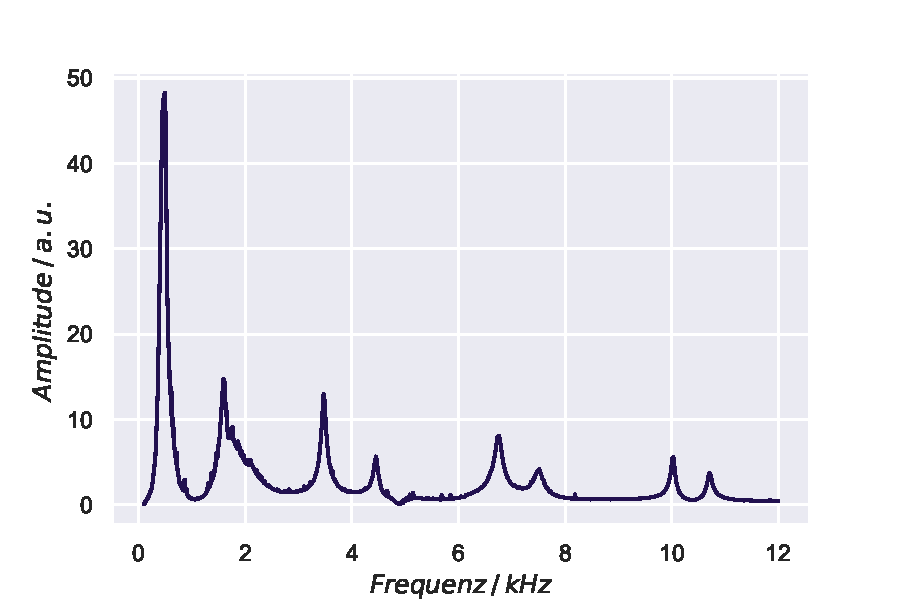
\includegraphics[width=0.5\textwidth]{Daten/Festkörper/FK1_16mm_1.pdf} &   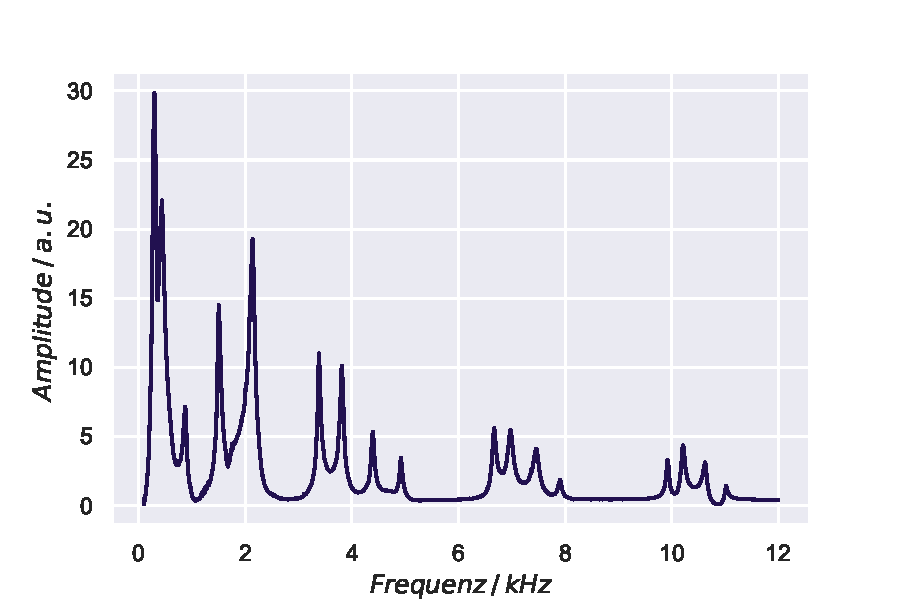
\includegraphics[width=0.5\textwidth]{Daten/Festkörper/FK1_16mm_3.pdf} \\
  (a) 2 Zylinder & (b) 4 Zylinder \\[6pt]
  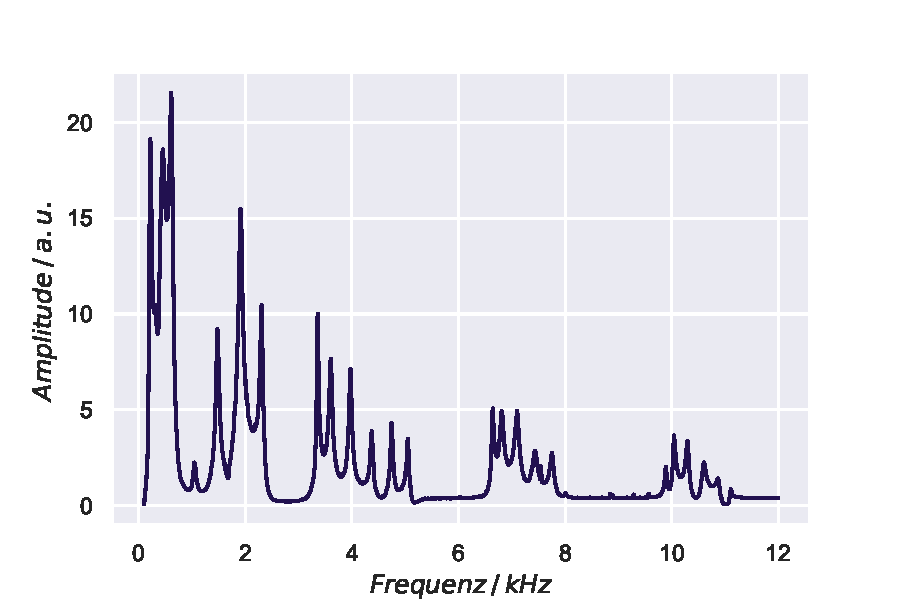
\includegraphics[width=0.5\textwidth]{Daten/Festkörper/FK1_16mm_5.pdf} &   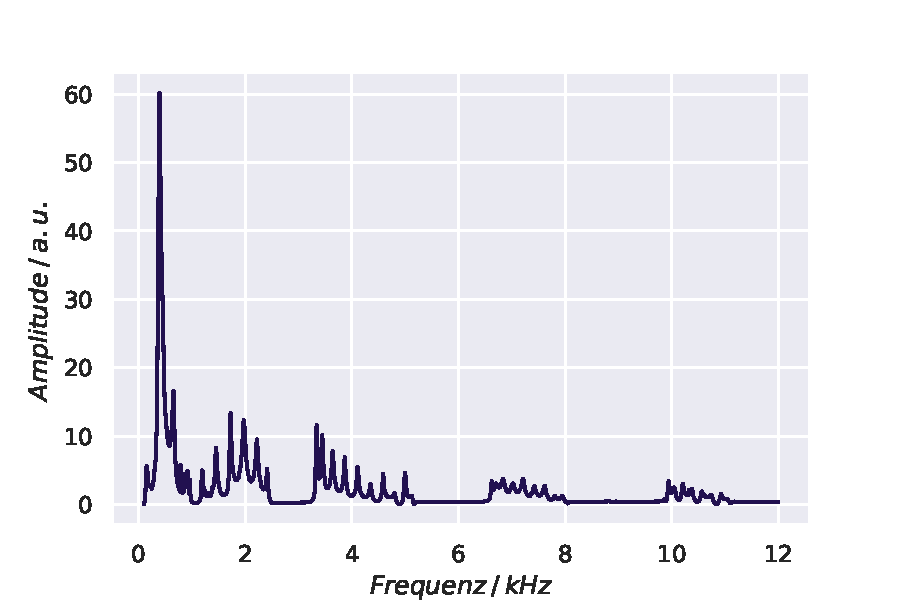
\includegraphics[width=0.5\textwidth]{Daten/Festkörper/FK1_16mm_9.pdf} \\
  (c) 6 Zylinder & (d) 10 Zylinder \\[6pt]
  
  \end{tabular}
  \caption{Die Frequenzspektren der Zylinderketten verschiedener Länge bei einem Irisdurchmesser von $16\, \si{\milli\metre}$} 
  \label{fig:fk1}
\end{figure}
\subsubsection{Blenden verschiedener Durchmesser zwischen den Zylindern in der Resonatorkette}

Das Frequenzspektrum der Resonatorkette mit $2$,$4$ und $10$ Zylindern wurden erneut aufgenommen wobei dieses Mal der Durchmesser der Blenden variiert wurde. 
Die der Vergleich der Frequenzspektren mit verschiedene Blendendurchmesser ist für die Kette aus 10 Zylindern in der Abbildung \ref{fig:fkvergleich} gezeigt. \\
Es ist zunächst zu bemerken, dass die Abstände der Peaks für größere Durchmesser vergrößern. Verbunden mit dem größeren Abstand zwischen den Peaks ist auch ein kleinerer Abstand zwischen den Bändern. Mit größerem Blendendurchmesser wird die Kette einem Aufbau ohne Blenden immer ähnlicher. 
Die unterschiedlichen Abstände liegen an der veränderten Kopplung zwischen den einzelnen Resonatoren. 
Des Weiteren haben die Peaks der ersten Ordnungen für Blenden mit größerem Durchmesser eine höhere Amplitude. Die somit werden die Peaks erster Ordnungen durch kleinere Blendendurchmesser unterdrückt. 

\begin{figure}[H]
  \centering
  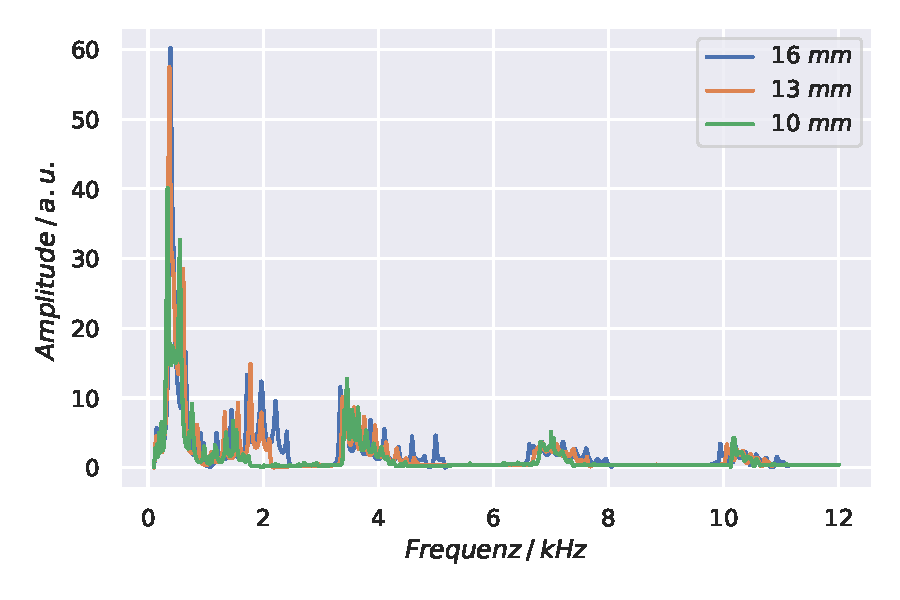
\includegraphics[width=0.8\textwidth]{Daten/Festkörper/vergleich.pdf}
  \caption{Vergleich zwischen den Frequenzspektren der Zylinderketten mit verschiedenen Irisdurchmesser.}
  \label{fig:fkvergleich}
\end{figure}
\subsubsection{Modifikation der Resonatorkette}

In vorher betrachteten Ketten hatten alle Zylinder die selbe Länge. 
Dieser Abschnitt wird untersucht, welchen Einfluss Variationen in der Kette haben. \\
Zunächst wurden die Frequenzspektren der Resonatorketten mit drei verschiedenen Defekten, also Zylinder mit unterschiedlicher Länge in der Kette, aufgenommen und in der Abbildung \ref{fig:fkMod} mit dem Spektrum der Kette ohne ein Defekt verglichen. \\
Es ist zunächst zu erkennen, dass sich die Bänder durch das Einfügen eines Defektes verschoben haben. Die Resonanzen liegen somit innerhalb der Bandlücken des Spektrums ohne ein Defekt. In der dritten Abbildung \ref{fig:fkMod}c) ist ebenfalls noch zu erkennen, dass sich neue Resonanzen in den Lücken bilden und so das Band füllen. 


\begin{figure}[H]
  \centering
  \begin{tabular}{cc}

  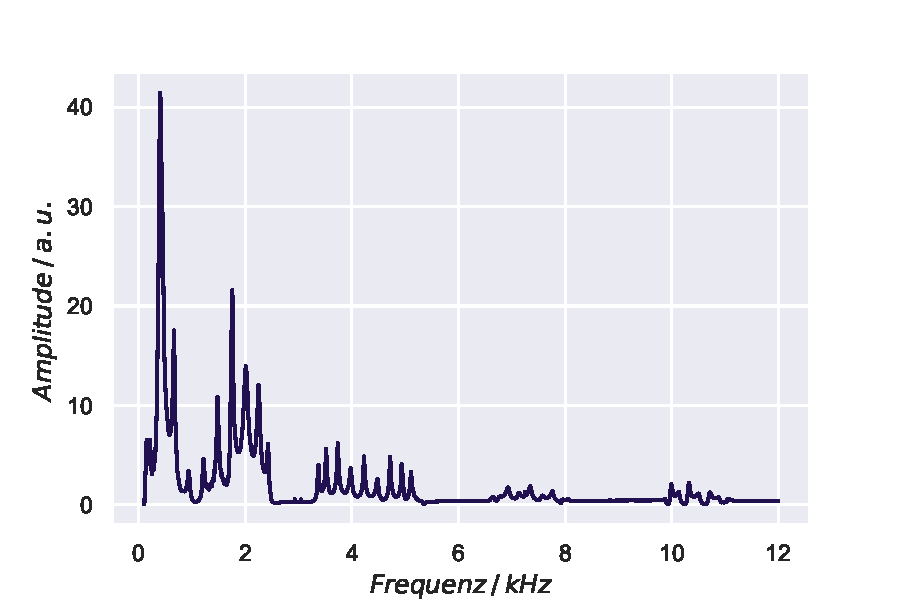
\includegraphics[width=0.5\textwidth]{Daten/Festkörper/FK3_16mm_37-5mm.pdf} &   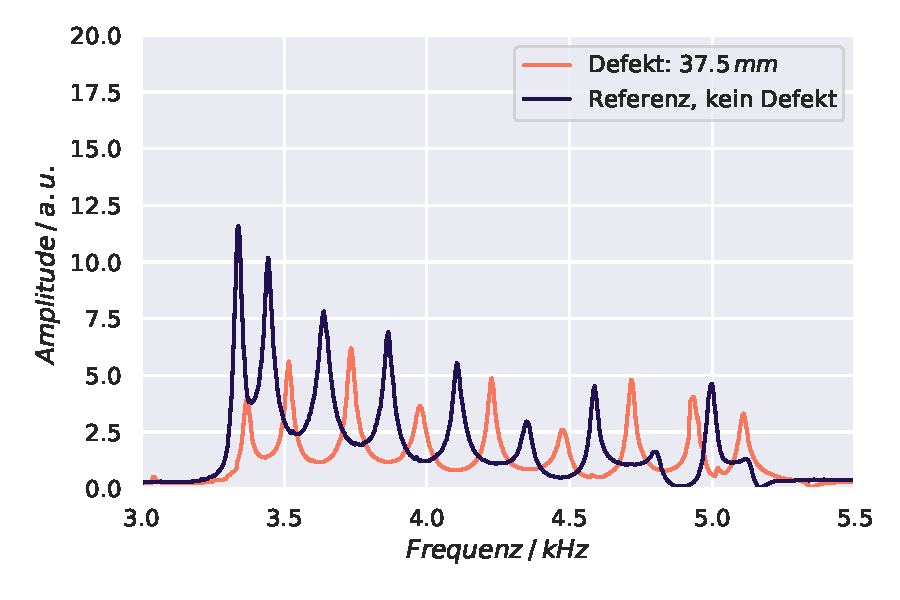
\includegraphics[width=0.5\textwidth]{Daten/Festkörper/FK3_16mm_37-5mmZOOM.pdf} \\
  \multicolumn{2}{c}{(a)  $37.5 \,\si{\milli\metre}$ Zylinder als Defekt}\\[6pt]
  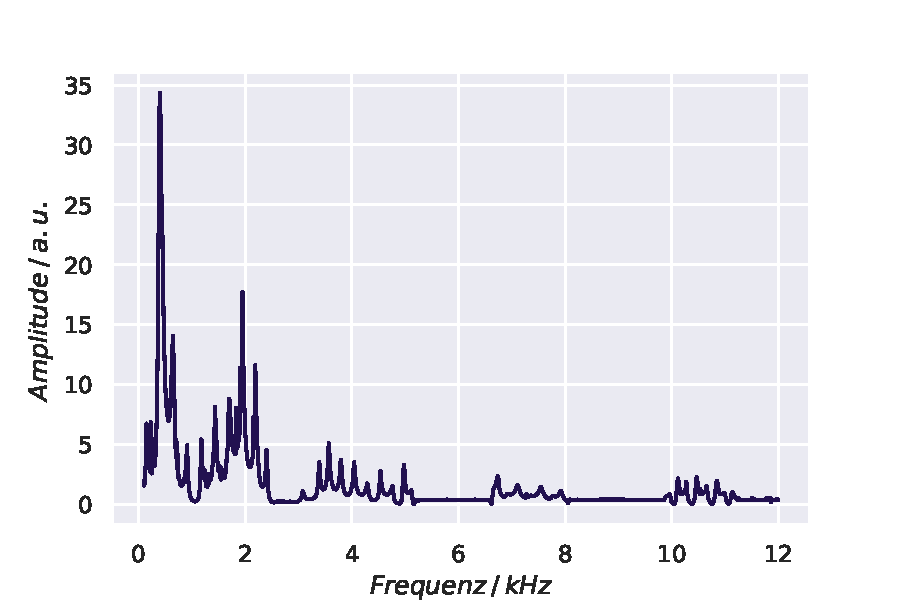
\includegraphics[width=0.5\textwidth]{Daten/Festkörper/FK3_16mm_62-5mm.pdf} &   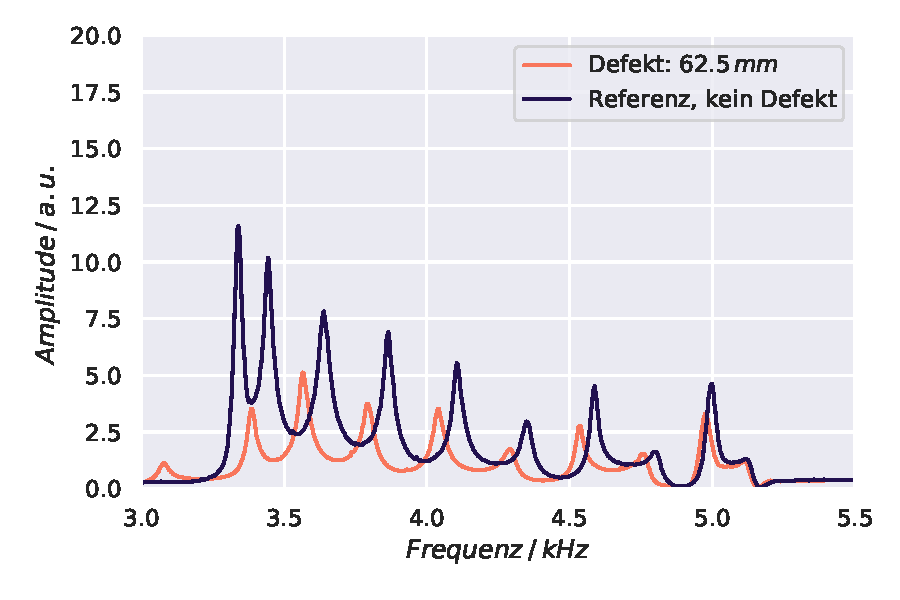
\includegraphics[width=0.5\textwidth]{Daten/Festkörper/FK3_16mm_62-5mmZOOM.pdf} \\
  \multicolumn{2}{c}{(b)  $62.5 \,\si{\milli\metre}$ Zylinder als Defekt}\\[6pt]
  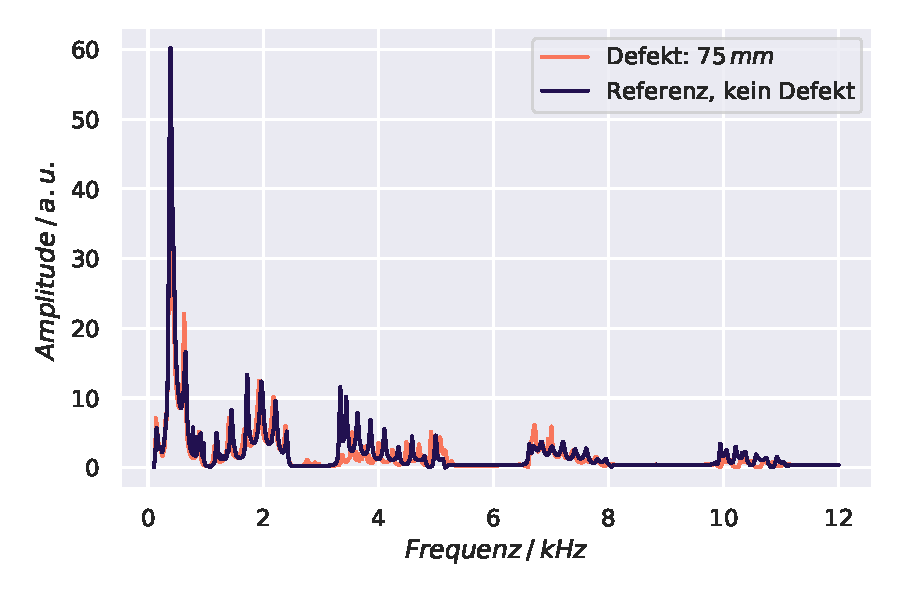
\includegraphics[width=0.5\textwidth]{Daten/Festkörper/FK3_16mm_75mm.pdf} &   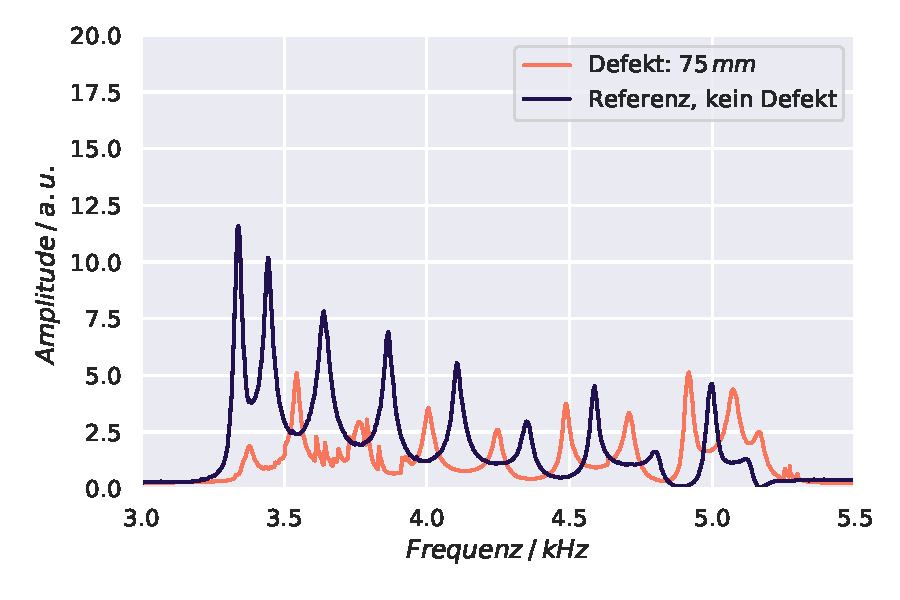
\includegraphics[width=0.5\textwidth]{Daten/Festkörper/FK3_16mm_75mmZOOM.pdf} \\
  \multicolumn{2}{c}{(c)  $75 \,\si{\milli\metre}$ Zylinder als Defekt}\\[6pt]
  
  \end{tabular}
  \caption{Auswirkungen eines Defekts in der Resonatorkette auf das Frequenzspektrum. Die rechten Plots zeigen den Zoom auf das zweite Band.} 
  \label{fig:fkMod}
\end{figure}
Für die folgende Analyse wurde die Kette so aufgebaut, dass sie alternierend Zylinder der Länge $50\,\si{\milli\metre}$ bzw. $75\,\si{\milli\metre}$ besitzt. Das Frequenzspektrum dieser alternierenden Kette wurde in Abbildung 
\ref{fig:fkMod2} mit dem Spektrum eines einzelnen $50\,\si{\milli\metre}$ bzw. $75\,\si{\milli\metre}$ Zylinders verglichen. \\
Das Frequenzspektrum der alternierenden Kette zeigt große Unterschiede im Vergleich mit den zuvor betrachteten Spektren. Die Resonanzen sind erneut verschoben jedoch fallen die Bänder zusätzlich kaum mit den Resonanzen der einzelnen Zylinder zusammen. 
Stattdessen sind die Bänder der alternierenden Kette innerhalb der Bandlücken der einzelnen Zylinder zu finden. Dies ist damit zu erklären, dass die Aneinanderreihung der Zylinder zu destruktiver Interferenz an den Resonanzen führt. Es kann nur zu Resonanzen in der alternierenden Kette kommen, wenn nicht beide Zylindertypen die Resonanzen des jeweils anderen Typen stark unterdrücken. 
Dies ist der Fall bei dem Band um die Frequenz $7000 \, \si{\hertz}$. Hier liegen überlappen sich die Resonaznen der einzelnen Zylinder, es kommt zu keiner destruktiven Interferrenz und somit kann sich an dieser Stelle ein Band im Gesamtsystem bilden. \\ 

\begin{figure}[H]
  \centering
  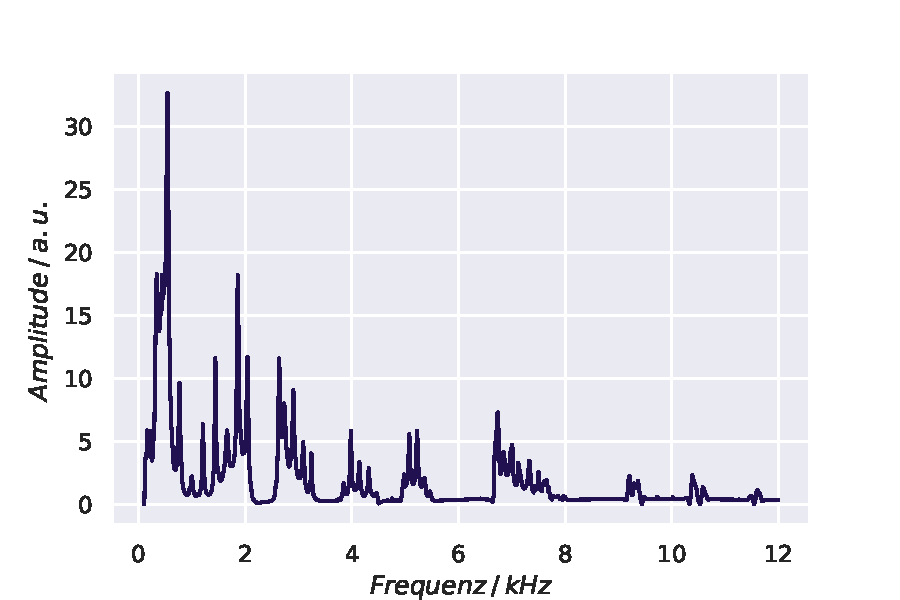
\includegraphics[width=0.7\textwidth]{Daten/Festkörper/FK4.pdf} 
  \caption{Vergleich zwischen dem Frequenzspektrum der Resonatorkette mit abwechselnder Zylinderlänge und dem Spektrum der einzelnen Zylinder.} 
  \label{fig:fkMod2}
\end{figure}
Abschließend wird nun das Frequenzspektrum einer Kette aus acht $50\,\si{\milli\metre}$ Zylinder mit alternierenden Blendendurchmesser ($16\, mm$ und $13\, mm$) gemessen. Die Ergebnisse sind in den Abbildungen \ref{fig:fkMod3} wiedergegeben. Zum Vergleich wurde ebenfalls das Spektrum der selben Kette mit ausschließlich $16\, mm$ Blenden dargestellt. \\
Hier verschieben sich die Bänder nicht. Trotzdem unterscheidet sich die Struktur wesentlich von der Struktur des Referenzspektrums. Insbesondere haben sich kleine Bandlücken innerhalb der Bänder aufgespalten. Die deutlich erkennbaren Bandlücken sind in der Abbildung orange markiert. 
Die variierenden Blenden beeinflussen somit die Dispersionsrelation und die allgemeine Bandstruktur des simulierten Festkörpers. 

\begin{figure}[H]
  \centering
  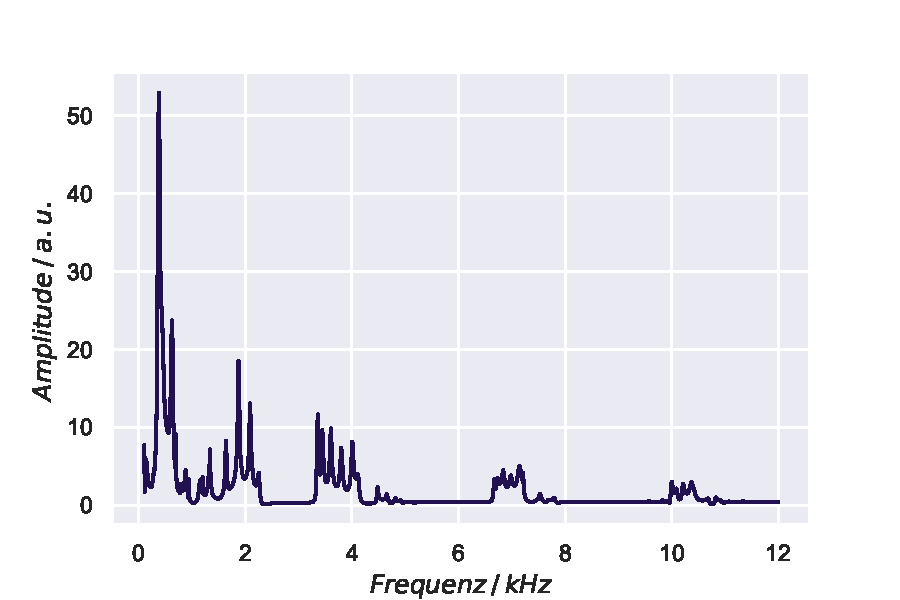
\includegraphics[width=0.7\textwidth]{Daten/Festkörper/FK5.pdf} 
  \caption{Vergleich zwischen dem Frequenzspektrum der Resonatorkette mit abwechselnden Blendendurchmesser und dem Spektrum der Kette mit ausschließlich $16\, mm$ Blenden.} 
  \label{fig:fkMod3}
\end{figure}